%%
%% This is file `./samples/longsample.tex',
%% generated with the docstrip utility.
%%
%% The original source files were:
%%
%% apa7.dtx  (with options: `longsample')
%% ----------------------------------------------------------------------
%% 
%% apa7 - A LaTeX class for formatting documents in compliance with the
%% American Psychological Association's Publication Manual, 7th edition
%% 
%% Copyright (C) 2021 by Daniel A. Weiss <daniel.weiss.led at gmail.com>
%% 
%% This work may be distributed and/or modified under the
%% conditions of the LaTeX Project Public License (LPPL), either
%% version 1.3c of this license or (at your option) any later
%% version.  The latest version of this license is in the file:
%% 
%% http://www.latex-project.org/lppl.txt
%% 
%% Users may freely modify these files without permission, as long as the
%% copyright line and this statement are maintained intact.
%% 
%% This work is not endorsed by, affiliated with, or probably even known
%% by, the American Psychological Association.
%% 
%% ----------------------------------------------------------------------
%% 
\documentclass[man]{apa7}

\usepackage{lipsum}

\usepackage[american]{babel}

\usepackage{csquotes}
\usepackage[style=apa,backend=biber]{biblatex}
\addbibresource{bibliography.bib}

\title{Sample APA-Style Document Using the \textsf{apa7} Package}
\shorttitle{Sample Document}

\authorsnames{Daniel A. Weiss}
\authorsaffiliations{A University Somewhere}

\leftheader{Weiss}

\abstract{\lipsum[1]}

\keywords{APA style, demonstration}

\authornote{
   \addORCIDlink{Daniel A. Weiss}{0000-0000-0000-0000}

  Correspondence concerning this article should be addressed to Daniel A. Weiss, Department of Educational Psychology, Counseling and
  Special Education, A University Somewhere, 123 Main St., Oneonta, NY
  13820.  E-mail: daniel.weiss.led@gmail.com}

\begin{document}
\maketitle
\lipsum[2]

\Textcite{vonDavier2011} said this,
too \parencite{vonDavier2011,Lassen2006}.  Further evidence comes from
other sources \parencite{Shotton1989,Lassen2006}.  \lipsum[3]

\section{Method}
\subsection{Participants}
\lipsum[4]

\subsection{Materials}
\lipsum[5]

\subsection{Design}
\lipsum[6]

\subsection{Procedure}
\lipsum[7]

\subsubsection{Instrument \#1}
\lipsum[8]

\paragraph{Reliability}
\lipsum[9]

\subparagraph{Inter-rater reliability}
\lipsum[10]

\subparagraph{Test-retest reliability}
\lipsum[11]

\paragraph{Validity}
\lipsum[12]

\subparagraph{Face validity}
\lipsum[13]

\subparagraph{Construct validity}
\lipsum[14]

\section{Results}
Table~\ref{tab:BasicTable} summarizes the data. \lipsum[15]

\begin{table}
  \caption{Sample Basic Table}
  \label{tab:BasicTable}
  \begin{tabular}{@{}llr@{}}         \toprule
  \multicolumn{2}{c}{Item}        \\ \cmidrule(r){1-2}
  Animal    & Description & Price \\ \midrule
  Gnat      & per gram    & 13.65 \\
            & each        &  0.01 \\
  Gnu       & stuffed     & 92.50 \\
  Emu       & stuffed     & 33.33 \\
  Armadillo & frozen      &  8.99 \\ \bottomrule
  \end{tabular}
\end{table}

\begin{figure}
    \caption{This is my first figure caption.}
    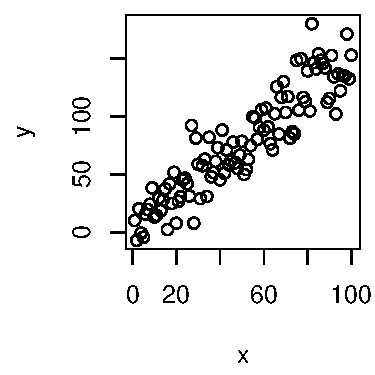
\includegraphics[bb=0in 0in 2.5in 2.5in, height=2.5in, width=2.5in]{Figure1.pdf}
    \figurenote{This is a great figure.}
    \label{fig:Figure1}
\end{figure}

Figure~\ref{fig:Figure1} shows this trend. \lipsum[16]

\section{Discussion}
\lipsum[17]

\lipsum[18]

\lipsum[19]

\printbibliography

\appendix

\section{Instrument}
\label{app:instrument}

As shown in Figure~\ref{fig:Figure2}, these results are impressive. \lipsum[20]

\begin{figure}
    \caption{This is my second figure caption.}
    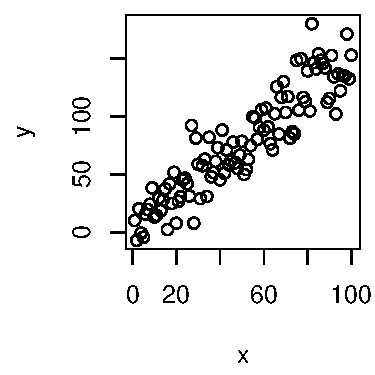
\includegraphics[bb=0in 0in 2.5in 2.5in, height=2.5in, width=2.5in]{Figure1.pdf}
    \figurenote{This is a great appendix figure.}
    \label{fig:Figure2}
\end{figure}

\lipsum[21]
\section{Pilot Data}
\label{app:surveydata}

The detailed results are shown in Table~\ref{tab:DeckedTable}. \lipsum[22]

\begin{table}
  \begin{threeparttable}
    \caption{A More Complex Decked Table}
    \label{tab:DeckedTable}
    \begin{tabular}{@{}lrrr@{}}         \toprule
    Distribution type  & \multicolumn{2}{l}{Percentage of} & Total number   \\
                       & \multicolumn{2}{l}{targets with}  & of trials per  \\
                       & \multicolumn{2}{l}{segment in}    & participant    \\ \cmidrule(r){2-3}
                                    &  Onset  &  Coda            &          \\ \midrule
    Categorical -- onset\tabfnm{a}  &    100  &     0            &  196     \\
    Probabilistic                   &     80  &    20\tabfnm{*}  &  200     \\
    Categorical -- coda\tabfnm{b}   &      0  &   100\tabfnm{*}  &  196     \\ \midrule
    \end{tabular}
    \tablenote{All data are approximate.

            \tabfnt{a}Categorical may be onset.
            \tabfnt{b}Categorical may also be coda.

            \tabfnt{*}\textit{p} < .05.
            \tabfnt{**}\textit{p} < .01.
         }
  \end{threeparttable}
\end{table}

\lipsum[23]

\end{document}

%% 
%% Copyright (C) 2021 by Daniel A. Weiss <daniel.weiss.led at gmail.com>
%% 
%% This work may be distributed and/or modified under the
%% conditions of the LaTeX Project Public License (LPPL), either
%% version 1.3c of this license or (at your option) any later
%% version.  The latest version of this license is in the file:
%% 
%% http://www.latex-project.org/lppl.txt
%% 
%% Users may freely modify these files without permission, as long as the
%% copyright line and this statement are maintained intact.
%% 
%% This work is not endorsed by, affiliated with, or probably even known
%% by, the American Psychological Association.
%% 
%% 
%% This work is "maintained" (as per LPPL maintenance status) by
%% Daniel A. Weiss.
%% 
%% This work consists of the file  apa7.dtx
%% and the derived files           apa7.ins,
%%                                 apa7.cls,
%%                                 apa7.pdf,
%%                                 README,
%%                                 APA7american.txt,
%%                                 APA7british.txt,
%%                                 APA7dutch.txt,
%%                                 APA7english.txt,
%%                                 APA7french.txt,
%%                                 APA7german.txt,
%%                                 APA7ngerman.txt,
%%                                 APA7greek.txt,
%%                                 APA7czech.txt,
%%                                 APA7turkish.txt,
%%                                 APA7endfloat.cfg,
%%                                 Figure1.pdf,
%%                                 shortsample.tex,
%%                                 longsample.tex, and
%%                                 bibliography.bib.
%% 
%%
%% End of file `./samples/longsample.tex'.
